\documentclass[document.tex]{subfiles} 
\begin{document}

\clearpage
\subsection{Условно-графическое обозначение}
Адаптер, позволяющий выводить условно графические изображения, именуется
ElectronicSymbolAdapter и имеет определение, представленное в
листинге~\ref{lst:symbol}.

\begin{listing}[ht]
\begin{minted}[linenos=true]{python}
class ElectronicSymbolAdapter(AbstractAdapter):
    public_properties = ('image',)
    default_content_type = 'image/png'

    def default_method(self):
        image = self.image
        large_image = Image.new('RGB', (600, 400), self._options['background'])
        large_image.paste(image,
                          (300 - self._options['width'] / 2,
                           200 - self._options['height'] / 2))
        _, tmpfile = mkstemp(suffix='.png')
        large_image.save(tmpfile)
        return tmpfile
\end{minted}
\caption{Программное описание класса адаптера УГО}
\label{lst:symbol}
\end{listing}

Пример применения адаптера УГО к устройству (в данном случае,
демультиплексор) иллюстрируется кодом, представленном в
листинге~\ref{lst:symbolgen}.

\begin{listing}[ht]
\begin{minted}{pycon}
>>> from circuitry.adapters.visual.symbol import ElectronicSymbolAdapter
>>> from circuitry.devices.mux import DeviceDemux
>>>
>>> device_demux = DeviceDemux(strobe_signals='v:1', address_signals='a:2',
...                            data_signals='d:1', output_signals='o:4',
...                            strobe_signals_subs=dict(v0=1),
...                            data_signals_subs=dict(d0=1),
...                            output_signals_subs=dict(o0=1, o1=1, o2=1, o3=1))
>>>
>>> ElectronicSymbolAdapter(device_demux).default_method()
'/tmp/tmp8y85m2.png'
\end{minted}
\caption{Генерация условно-графического обозначения}
\label{lst:symbolgen}
\end{listing}

\clearpage
Файл, полученный применением адаптера представлен на
рис.~\ref{fig:adapters_symbol}.

\begin{figure}[here]
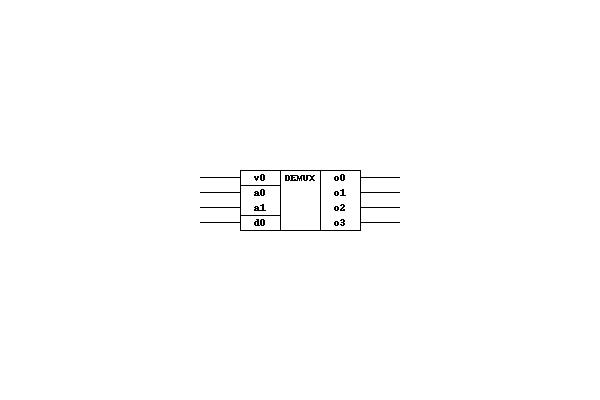
\includegraphics[width=1\linewidth]{adapters_symbol}
\caption{Условно-графическое обозначение демультиплексора}
\label{fig:adapters_symbol}
\end{figure}

\end{document}